\documentclass[../main]{subfiles}

\begin{document}
%%%%%%%%%%%%%%%%%%%%%%%%%%%%%%%%%%%%%%%%%%%%%%%%%%%%%%%%%%%%%%%%%%%%%%%%%
\graphicspath{{images/}}
% To get the right chapter number
\ifSubfilesClassLoaded{
    \externaldocument[main-]{../main}
    \setcounterref{chapter}{main-chap:hello-turtle}
    \addtocounter{chapter}{-1}
    \setcounter{page}{\getpagerefnumber{main-chap:hello-turtle}}
}{}
%%%%%%%%%%%%%%%%%%%%%%%%%%%%%%%%%%%%%%%%%%%%%%%%%%%%%%%%%%%%%%%%%%%%%%%%%
\pagestyle{mypagestyle}
\chapterstyle{MyChapterStyle}  

\chapter{Hello, Turtle!}
\label{chap:hello-turtle}

\begin{objectivesbox}
    \begin{objectiveslist}
        \item hoe je de turtle module importeert en een schildpad aanmaakt;
        \item met welke functies je de schildpad kunt besturen;
        \item met welke functies je de pen van de schildpad kunt bedienen;
        \item hoe je met penkleuren en vulkleuren kunt werken;
        \item hoe je cirkels en stippen kunt tekenen met de schildpad.
    \end{objectiveslist}
\end{objectivesbox}

Een \emph{algoritme} is een reeks instructies die leidt tot een einddoel. Eenvoudiger gezegd is een algoritme een stappenplan. Wellicht denk je bij algoritmen meteen aan computers, maar dat hoeft niet. In het dagelijks leven gebruik je bewust of onbewust allerlei algoritmen. Bijvoorbeeld om je tanden te poetsen:
\begin{minipage}[t]{0.6\linewidth}
\begin{enumerate}[itemsep=0pt, parsep=2pt]
\item Draai de kraan open.
\item Spoel je mond.
\item Pak je tandenborstel.
\item Spoel je tandenborstel af.
\item Pak de tandpasta.
\item Draai het dopje van de tandpasta los.
\item … enzovoort
\end{enumerate}
\end{minipage}\hfill
\begin{minipage}[t]{0.3\linewidth}
\adjustimage{width=0.9\linewidth, valign=T}{tandenpoetsen}
\end{minipage}

\vspace{\baselineskip}
In dit hoofdstuk ga je aan de slag met algoritmen om in Python een schildpad (Engels: turtle) te besturen.

\section{Python Turtle}
\label{sec:python_turtle}

Start in Mu editor met een nieuw bestand door op de knop \menu{New} te klikken. Sla het bestand op als \file{hello\_turtle.py} in je \folder{Pythonprojecten/Oefeningen} map. Typ de code die je hieronder in listing~\ref{lst:hello-turtle-01} ziet in het bestand en let daarbij goed op het verschil tussen hoofdletters en kleine letters!

\begin{python}[style=mu, caption={\file{hello\_turtle.py}}, label={lst:hello-turtle-01}]
import turtle

tony = turtle.Turtle()

tony.forward(100)
\end{python}

Run de code om het resultaat te bekijken. Krijg je een foutmelding? Controleer dan of je de code exact hebt overgetypt. Als je het goed hebt gedaan, zou je het resultaat zoals in figuur~\ref{fig:hello_turtle_01} moeten zien.

\begin{figure}[b]
    \centering
    \adjustimage{width=0.5\linewidth}{turtle_01}
    \caption{Output van listing~\ref{lst:hello-turtle-01}}
    \label{fig:hello_turtle_01}
\end{figure}

Sommige functies zoals \texttt{print()} zitten standaard in Python, maar om met de schildpad te kunnen werken is het nodig de module \texttt{turtle} te importeren. Dat gebeurt op regel 1. Op regel 3 maken we met de functie \texttt{Turtle()} uit de \texttt{turtle} module een schildpad aan met de naam \texttt{tony}. Op regel 5 sturen we \texttt{tony} 100 pixels naar voren.

Waarom hebben we het eigenlijk telkens over een schildpad? Onze Tony lijkt helemaal niet op een schildpad! Hij lijkt meer op een pijlpunt! Daar gaan we verandering in brengen. En we gaan hem ook van richting laten veranderen. Pas je code aan zodat hij overeenkomt met listing~\ref{lst:hello-turtle-02}. Maak daarbij handig gebruik van de code die je al hebt getypt. Je hoeft niet alles opnieuw te typen. Met de toetscombinaties \keys{Ctrl + C} en \keys{Ctrl + V} kun je coderegels kopiëren en plakken

\begin{python}[style=mu, caption={\file{hello\_turtle.py}}, label={lst:hello-turtle-02}]
import turtle

tony = turtle.Turtle()
tony.shape('turtle')

tony.forward(100)
tony.left(90)
tony.forward(50)
tony.left(90)
tony.forward(100)
tony.left(90)
tony.forward(50)
\end{python}

Run de code opnieuw. Je zou nu een schildpad moeten zien die een rechthoek tekent.

\begin{infobox}[Draaiingshoeken]
De waarde die je tussen de haakjes aan de functie \texttt{tony.forward()} meegeeft, is het aantal pixels dat de schildpad vooruit moet bewegen. Maar wat doet het getal \texttt{90} tussen de haakjes van \texttt{tony.left()}? Wellicht had je al bedacht dat dat het aantal graden is dat de schildpad naar links moet draaien. Een hoek van 90\textdegree{} is een rechte hoek. Dat betekent dat de schildpad na het draaien precies loodrecht op zijn oorspronkelijke richting staat. De aanroep \texttt{tony.left(90)} zorgt er dus voor dat de schildpad 90\textdegree{} naar links draait, oftewel linksaf slaat.

\begin{center}
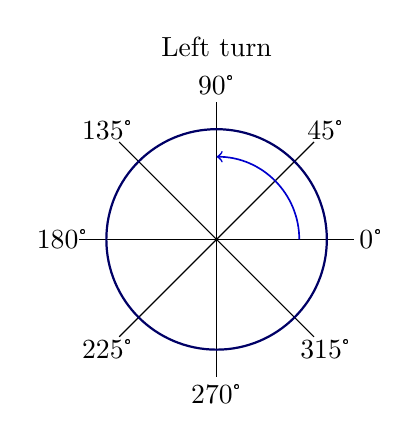
\begin{tikzpicture}[scale=0.7]
    \foreach \angle in {0, 45, 90, 135, 180, 225, 270, 315} {
        \draw (0, 0) -- (\angle:2.5cm) node at (\angle:2.8cm) {\angle\textdegree};
    }
    \draw [thick, draw=blue!40!black] (0, 0) circle [radius=2cm];
    \draw [->, semithick, draw=blue!80!black] (1.5, 0) arc [start angle=0, end angle=90, radius=1.5cm];
    \node at (0, 3.5) {Left turn};
\end{tikzpicture}
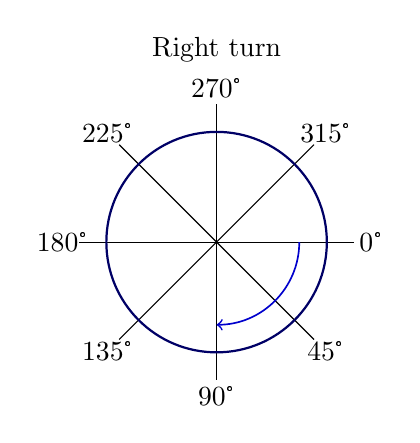
\begin{tikzpicture}[scale=0.7]
    \foreach \angle in {0, 45, 90, 135, 180, 225, 270, 315} {
        \draw (0, 0) -- (-\angle:2.5cm) node at (-\angle:2.8cm) {\angle\textdegree};
    }
    \draw [thick, draw=blue!40!black] (0, 0) circle [radius=2cm];
    \draw [->, semithick, draw=blue!80!black] (1.5, 0) arc [start angle=0, end angle=-90, radius=1.5cm];
    \node at (0, 3.5) {Right turn};
\end{tikzpicture}
\end{center}
\end{infobox}
%%%%%%%%%%%%%%%%%%%%%%%%%%%%%%%%%%%%%%%
\subsection*{Opgaven}

\begin{opgave}[icons={laptop, pen}]
\begin{qlist}
\item Wijzig de code in \file{hello\_turtle.py} zodanig, dat de schildpad een vierkant tekent in plaats van een rechthoek.
\item Laat de schildpad een gelijkzijdige driehoek tekenen. Dat is een driehoek met drie even lange zijden en hoeken van 60\textdegree{}.
\begin{center}
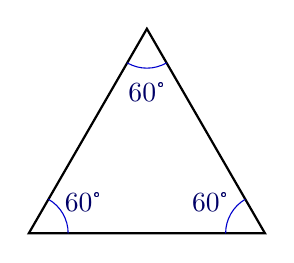
\begin{tikzpicture}
    \draw [thick] (0, 0) -- (3, 0) -- (60:3) -- cycle;
    \draw [blue!80!black] (0.5, 0) arc [start angle=0, end angle=60, radius=0.5cm];
    \draw [blue!80!black] ([shift={(3,0)}]120:0.5) arc [start angle=120, end angle=180, radius=0.5cm];
    \draw [blue!80!black] ([shift={(60:3)}]240:0.5) arc [start angle=240, end angle=300, radius=0.5cm];
    \node [text=blue!40!black] at (30:.8) {60\textdegree};
    \node [text=blue!40!black] at ([shift={(150:.8)}]3,0) {60\textdegree};
    \node [text=blue!40!black] at ([shift={(270:.8)}]60:3) {60\textdegree};
\end{tikzpicture}
\end{center}
\item Je hebt waarschijnlijk gemerkt dat bij vraag b de aanroep \texttt{tony.left(60)} niet het gewenste resultaat oplevert. Welke draaiingshoek moet je gebruiken om een gelijkzijdige driehoek te tekenen? Leg uit waarom.\par
{\setlength{\parskip}{.8cm}\hruled\par\hruled\par\hruled}
\end{qlist}
\end{opgave}
%--------------------------------------
\begin{antwoord}
\begin{qlist}
\item
\begin{python}[style=mu]
import turtle

tony = turtle.Turtle()
tony.shape('turtle')

tony.forward(100)
tony.left(90)
tony.forward(100)
tony.left(90)
tony.forward(100)
tony.left(90)
tony.forward(100)
\end{python}
\item
\begin{python}[style=mu]
import turtle

tony = turtle.Turtle()
tony.shape('turtle')

tony.forward(100)
tony.left(120)
tony.forward(100)
tony.left(120)
tony.forward(100)
\end{python}
\item Om een gelijkzijdige driehoek te tekenen, moet je de schildpad 120\textdegree{} laten draaien. Dat is het verschil tussen 180\textdegree{} (een halve draai) en 60\textdegree{} (de hoek van de driehoek). Je kunt ook zeggen dat 360\textdegree{} gedeeld door 3 (het aantal zijden van de driehoek) gelijk is aan 120\textdegree{}.

\begin{center}
\begin{tikzpicture}
    \draw [thick] (0, 0) -- (3, 0) -- (60:3);
    \draw [dashed, -{Stealth[length=5mm]}] (3, 0) -- (4, 0);
    \draw [dashed] (4, 0) -- (6, 0);
    \draw [blue!80!black] ([shift={(3,0)}]120:0.5) arc [start angle=120, end angle=180, radius=0.5cm];
    \node [text=blue!40!black] at ([shift={(150:.8)}]3,0) {60\textdegree};
    \draw [dotted, ->] (4, 0) arc [start angle=0, end angle=120, radius=1cm];
    \node [font=\large] at ([shift={(50:1.5)}]3,0) {120\textdegree};
\end{tikzpicture}
\end{center}
\end{qlist}
\end{antwoord}
%%%%%%%%%%%%%%%%%%%%%%%%%%%%%%%%%%%%%%%
\section{De basisbewegingen}%
\label{sec:basisbewegingen}

Tot nu toe hebben we in onze code voor de beweging van de schilpad de functies \texttt{forward()} en \texttt{left()} gebruikt. Kun je voorspellen welke bewegingsfuncties er nog meer zijn? Juist, \texttt{backward()} en \texttt{right()}. Omdat je deze vier functies heel vaak gebruikt, zijn er afkortingen voor, zodat je minder hoeft te typen. In tabel~\ref{tbl:basisbewegingen} zie je een overzicht van de basisbewegingen van de schildpad, inclusief de afkortingen en een korte uitleg van wat ze doen. In plaats van \texttt{tony.forward(100)} kun je dus ook \texttt{tony.fd(100)} typen. Dat scheelt weer een paar toetsaanslagen!

\begin{table}[ht]
    \centering
    \begin{tblr}{
        colspec={Q[l]Q[l]Q[l]},
        column{1,2} = {font=\ttfamily},
        row{1} = {font=\sffamily\bfseries},
        stretch=1.5}
        \topline
        Functie & Afkorting & Werking\\
        \clinels{1}\clinems{2}\cliners{3}
        forward(\textit{distance}) & fd(\textit{distance}) & Ga \texttt{\textit{distance}} vooruit.\\
        backward(\textit{distance}) & bk(\textit{distance}) & Ga \texttt{\textit{distance}} achteruit.\\
        left(\textit{angle}) & lt(\textit{angle}) & Draai \texttt{\textit{angle}}\textdegree{} naar links.\\
        right(\textit{angle}) & rt(\textit{angle}) & Draai \texttt{\textit{angle}}\textdegree{} naar rechts.\\
        \bottomline
    \end{tblr}
    \caption{Basisbewegingen van de schildpad}
    \label{tbl:basisbewegingen}
\end{table}

Merk op dat je turtlefuncties moet aanroepen met de naam van de schildpad ervoor, gevolgd door een punt. Dus niet \texttt{rt(45)}, maar \texttt{tony.rt(45)}. Als je jouw schildpad een andere naam hebt gegeven, bijvoorbeeld \texttt{tina}, dan moet je \texttt{tina.rt(45)} typen (zie listing~\ref{lst:hello-turtle-03}).

\begin{python}[style=mu, caption={Hier heet de schildpad \texttt{tina}}, label={lst:hello-turtle-03}]
import turtle

tina = turtle.Turtle()

tina.rt(45)
tina.fd(80)
\end{python}
%%%%%%%%%%%%%%%%%%%%%%%%%%%%%%%%%%%%%%%
\subsection*{Opgaven}

\begin{opgave}[icons={laptop}]
Wijzig de code in \file{hello\_turtle.py} zodat hij overeenkomt met listing~\ref{lst:hello-turtle-04}. Run de code om te zien dat de schildpad het begin van een hoofdletter \textsf{H} tekent (figuur~\ref{fig:hello_turtle_02}).

\begin{python}[style=mu, caption={\file{hello\_turtle.py}}, label={lst:hello-turtle-04}]
import turtle

tony = turtle.Turtle()
tony.shape('turtle')

tony.lt(90)
tony.fd(100)
tony.bk(50)
tony.rt(90)
tony.fd(60)
\end{python}

\begin{figure}[ht]
    \centering
    \adjustimage{width=0.5\linewidth}{turtle_02}
    \caption{Output van listing~\ref{lst:hello-turtle-04}}
    \label{fig:hello_turtle_02}
\end{figure}

Maak de code af zodat een volledige hoofdletter \textsf{H} wordt getekend.
\end{opgave}
%--------------------------------------
\begin{antwoord}
\begin{python}[style=mu]
import turtle

tony = turtle.Turtle()
tony.shape('turtle')

tony.lt(90)
tony.fd(100)
tony.bk(50)
tony.rt(90)
tony.fd(60)
tony.lt(90)
tony.fd(50)
tony.bk(100)
\end{python}
\end{antwoord}
%%%%%%%%%%%%%%%%%%%%%%%%%%%%%%%%%%%%%%%
\section{Pen up, pen down en pen size}%
\label{sec:pen_up_down}

Zoals je hebt gemerkt, is \texttt{tony} een schildpad die van tekenen houdt, want hij heeft een pen vast waarmee hij zijn afgelegde weg tekent. Soms wil je echter dat \texttt{tony} zijn pen even van het `papier' haalt. Met de  functies \texttt{penup()} en \texttt{pendown()} kun je de pen van de schildpad bedienen (tabel~\ref{tbl:pen-bediening}). Wanneer de pen omhoog is, zal de schildpad niet tekenen als hij beweegt. 

\begin{table}[ht]
    \centering
    \begin{tblr}{
        colspec={Q[l]Q[l]Q[l]},
        column{1,2} = {font=\ttfamily},
        row{1} = {font=\sffamily\bfseries},
        stretch=1.5}
        \topline
        Functie & Afkortingen & Werking\\
        \clinels{1}\clinems{2}\cliners{3}
        penup() & pu()\textsf{,} up() & Til de pen omhoog.\\
        pendown() & pd()\textsf{,} down() & Zet de pen neer.\\
        \bottomline
    \end{tblr}
    \caption{Bediening van de pen}%
    \label{tbl:pen-bediening}
\end{table}

Daarnaast kun je de dikte van de pen instellen met de functie \texttt{pensize()}.

\begin{table}[ht]
    \centering
    \begin{tblr}{
        colspec={Q[l]Q[l]},
        column{1,2} = {font=\ttfamily},
        row{1} = {font=\sffamily\bfseries},
        stretch=1.5}
        \topline
        Functie & Werking\\
        \clinels{1}\cliners{2}
        pensize(\textit{width}) & Stel de dikte van de pen in op \textit{\texttt{width}}.\\
        \bottomline
    \end{tblr}
    \caption{Instelling van de pendikte}%
    \label{tbl:pen-dikte}
\end{table}

Bij de functies \texttt{penup()} en \texttt{pendown()} zet je niks tussen de haakjes, maar de functie \texttt{pensize()} heeft wél input nodig. Tussen de haakjes zet je een geheel getal dat de pendikte in pixels aangeeft. Dus bijvoorbeeld \texttt{tony.pensize(10)}.
%%%%%%%%%%%%%%%%%%%%%%%%%%%%%%%%%%%%%%%
\subsection*{Opgaven}

\begin{opgave}[icons={laptop}]
Breid je code in \file{hello\_turtle.py} uit zodat naast de letter \textsf{H} ook een hoofdletter \textsf{E} wordt getekend, met pendikte 5. Kies zelf mooie lengtes voor de drie horizontale lijnen van de letter \textsf{E}, zodat je resultaat lijkt op figuur~\ref{fig:hello_turtle_03}.

\begin{figure}[ht]
    \centering
    \adjustimage{width=0.5\linewidth}{turtle_03}
    \caption{De letters H en E met verschillende pendiktes}%
    \label{fig:hello_turtle_03}
\end{figure}

\begin{hints}
\item Na de code die de letter \textsf{H} tekent, moet je dus eerst \texttt{tony.penup()} aanroepen om de pen van het papier te halen. Vervolgens beweeg je de schildpad 20 pixels vooruit met \texttt{tony.fd(20)} (misschien moet je hem eerst nog draaien, zodat hij de goede kant op gaat). Daarna roep je \texttt{tony.pendown()} aan om de pen weer op het papier te zetten. Als je dat voor elkaar hebt, kun je de code maken die de letter \textsf{E} tekent.
\end{hints}
\end{opgave}
%--------------------------------------
\begin{antwoord}
\begin{python-breakable}[style=mu]
import turtle

tony = turtle.Turtle()
tony.shape('turtle')

# Letter H
tony.lt(90)
tony.fd(100)
tony.bk(50)
tony.rt(90)
tony.fd(60)
tony.lt(90)
tony.fd(50)
tony.bk(100)

tony.pu()
tony.rt(90)
tony.fd(20)
tony.pd()

# Letter E
tony.pensize(5)
tony.fd(60)
tony.bk(60)
tony.lt(90)
tony.fd(50)
tony.rt(90)
tony.fd(40)
tony.bk(40)
tony.lt(90)
tony.fd(50)
tony.rt(90)
tony.fd(60)
\end{python-breakable}
\end{antwoord}
%%%%%%%%%%%%%%%%%%%%%%%%%%%%%%%%%%%%%%%
\section{Kleuren}%
\label{sec:kleuren}

Onze schildpad tekent vooralsnog enkel zwarte lijnen; tijd voor wat fleurigheid! Uiteraard is er een functie om de penkleur van tony te veranderen.

\begin{table}[ht]
    \centering
    \begin{tblr}{
        colspec={Q[l]Q[l]},
        column{1,2} = {font=\ttfamily},
        row{1} = {font=\sffamily\bfseries},
        stretch=1.5}
        \topline
        Functie & Werking\\
        \clinels{1}\cliners{2}
        pencolor(\textit{color}) & Stel de kleur van de pen in op \textit{\texttt{color}}.\\
        \bottomline
    \end{tblr}
    \caption{Instelling van de penkleur}%
    \label{tbl:pen-kleur}
\end{table}

Tussen de haakjes van \texttt{pencolor()} zet je een kleur. De naam van de kleur is in het Engels en moet tussen aanhalingstekens staan. Dus bijvoorbeeld \texttt{tony.pencolor('yellow')} of \texttt{tony.pencolor('green')}. Andere kleuren zijn \texttt{gold}, \texttt{orange}, \texttt{red}, \texttt{maroon}, \texttt{violet}, \texttt{magenta}, \texttt{purple}, \texttt{navy}, \texttt{blue}, \texttt{skyblue}, \texttt{cyan}, \texttt{turquoise}, \texttt{lightgreen}, \texttt{darkgreen}, \texttt{chocolate}, \texttt{brown}, \texttt{black} en \texttt{gray}\footnote{Een complete lijst van de mogelijke kleuren vind je op \url{https://inventwithpython.com/blog/complete-list-tkinter-colors-valid-and-tested.html}}.
%%%%%%%%%%%%%%%%%%%%%%%%%%%%%%%%%%%%%%%
\subsection*{Opgaven}

\begin{opgave}[icons={laptop}]
Breid je code in \file{hello\_turtle.py} uit zodat de schildpad het woord \textsf{HELLO} tekent, waarbij elke letter een andere kleur en een andere pendikte heeft. Je mag zelf je favoriete kleuren en pendiktes kiezen. In figuur~\ref{fig:hello_turtle_04} zie je een voorbeeldje.

\begin{figure}[ht]
    \centering
    \adjustimage{width=0.6\linewidth}{turtle_HELLO}
    \caption{HELLO turtle}%
    \label{fig:hello_turtle_04}
\end{figure}

\begin{hints}
\item Om te voorkomen de tekst aan de rechterkant niet meer in het tekenvenster past, kun je de schildpad aan het begin van je code een stukje naar links laten bewegen. Bijvoorbeeld met \texttt{tony.up()}, \texttt{tony.bk(300)} en \texttt{tony.down()}.
\end{hints}
\end{opgave}
%--------------------------------------
\begin{antwoord}
*
\end{antwoord}
%%%%%%%%%%%%%%%%%%%%%%%%%%%%%%%%%%%%%%%
\begin{opgave}[icons={laptop}]
Klik op de \menu{New} knop om met een nieuw codebestand te starten. Sla het bestand op onder de naam \file{turtle\_house.py} in je \folder{oefeningen} map.\\
Importeer de \texttt{turtle} module en maak een schildpad aan. In \file{hello\_turtle.py} heette de schildpad \texttt{tony}, maar je mag hem nu een andere naam geven als je dat wilt.\\
Maak een algoritme dat het huisje in figuur~\ref{fig:turtle-house} tekent. In de figuur zie je hoe groot de binnenhoeken zijn, maar dat zijn niet de draaiingshoeken die je in je code moet gebruiken. Je zult zelf moeten berekenen welke draaiingshoeken nodig zijn om het huisje te tekenen.\\
Extra uitdaging: probeer het huisje te tekenen zonder de pen van het papier te halen en zonder meermaals hetzelfde lijnstuk te tekenen.
\begin{figure}[ht]
    \centering
    \adjustimage{width=0.5\linewidth}{turtle_house}
    \caption{Huisje}%
    \label{fig:turtle-house}
\end{figure}
\end{opgave}
%--------------------------------------
\begin{antwoord}
\begin{python-breakable}[style=mu]
import turtle

tony = turtle.Turtle()

tony.fd(80)     #onderzijde vierkant
tony.lt(90)
tony.fd(80)     #rechterzijde vierkant
tony.lt(90)
tony.fd(80)     #bovenzijde vierkant
tony.lt(90)
tony.fd(80)     #linkerzijde vierkant
tony.lt(135)
tony.fd(113)    #diagonaal
tony.lt(98)
tony.fd(50)     #rechterzijde dak
tony.lt(74)
tony.fd(50)     #linkerzijde dak
tony.lt(98)
tony.fd(113)    #diagonaal
\end{python-breakable}
\end{antwoord}
%%%%%%%%%%%%%%%%%%%%%%%%%%%%%%%%%%%%%%%%%
\section{Figuurvulling}%
\label{sec:figuurvulling}

Het is mogelijk om een door de turtle getekende figuur op te vullen met een kleur. Daarvoor gebruik je de volgende functies:

\begin{table}[ht]
    \centering
    \begin{tblr}{
        colspec={Q[l]Q[l]},
        column{1,2} = {font=\ttfamily},
        row{1} = {font=\sffamily\bfseries},
        stretch=1.5}
        \topline
        Functie & Werking\\
        \clinels{1}\cliners{2}
        fillcolor(\textit{color}) & Stel de vulkleur in op \textit{\texttt{color}}.\\
        begin\_fill() & Begin met het vullen van een figuur.\\
        end\_fill() & Stop met het vullen van een figuur.\\
        \bottomline
    \end{tblr}
    \caption{Functies voor figuurvulling}%
    \label{tbl:figuurvulling}
\end{table}

\begin{wrapfigure}{r}{2cm}
    \centering
    \adjustimage{width=0.9\linewidth}{filled_triangle}
    \caption{Een driehoek met vulling}%
    \label{fig:turtle-fill-01}   
\end{wrapfigure}
In listing~\ref{lst:turtle-fill-01} zie de code die nodig is om de driehoek in figuur~\ref{fig:turtle-fill-01} te tekenen. Je ziet dat de aanroep van \texttt{begin\_fill()} vóór het tekenen van de driehoek staat, en de aanroep van \texttt{end\_fill()} erna. De vulkleur is ingesteld op geel met de functie \texttt{fillcolor('yellow')}. Je kunt natuurlijk ook een andere kleur kiezen. Probeer het maar eens uit!

\begin{python}[style=mu, caption={\file{turtle\_fill.py}}, label={lst:turtle-fill-01}]
import turtle

tony = turtle.Turtle()
tony.shape('turtle')
tony.pensize(5)

# Stel de penkleur en de vulkleur in
tony.pencolor('black')
tony.fillcolor('yellow')

# Teken een driehoek met vulling
tony.begin_fill()
tony.fd(100)
tony.lt(120)
tony.fd(100)
tony.lt(120)
tony.fd(100)
tony.lt(120)
tony.end_fill()
\end{python}

%%%%%%%%%%%%%%%%%%%%%%%%%%%%%%%%%%%%%%%
\subsection*{Opgaven}

\begin{opgave}[icons={laptop}]
Als je nog geen codebestand \file{turtle\_fill.py} had gemaakt om listing~\ref{lst:turtle-fill-01} te testen, doe dat dan nu. Neem de code uit listing~\ref{lst:turtle-fill-01} over in \file{turtle\_fill.py} en run het bestand om te zien dat de driehoek met gele vulling wordt getekend.\\
Breid de code uit, zodat links van het driehoekje een regelmatige vijfhoek met rode vulling wordt getekend, zoals in figuur~\ref{fig:turtle-fill-02}. De zijden van de vijfhoek zijn 60 pixels lang.

\begin{figure}[ht]
    \centering
    \adjustimage{width=0.5\linewidth}{turtle_fill}
    \caption{Rode vijfhoek en gele driehoek}%
    \label{fig:turtle-fill-02}
\end{figure}
\end{opgave}
%--------------------------------------
\begin{antwoord}
In onderstaande uitwerking zijn de eerste coderegels weggelaten (let op de regelnummering).
\begin{python-breakable}[style=mu, firstnumber=11]
# Stel de penkleur en de vulkleur in
tony.pencolor('black')
tony.fillcolor('yellow')

# Teken een driehoek met vulling
tony.begin_fill()
tony.fd(100)
tony.lt(120)
tony.fd(100)
tony.lt(120)
tony.fd(100)
tony.lt(120)
tony.end_fill()

# Beweeg naar links
tony.pu()
tony.bk(150)
tony.pd()

# Stel de vulkleur in op rood
tony.fillcolor('red')

# Teken een vijfhoek met vulling
tony.begin_fill()
tony.fd(60)
tony.lt(72)
tony.fd(60)
tony.lt(72)
tony.fd(60)
tony.lt(72)
tony.fd(60)
tony.lt(72)
tony.fd(60)
tony.lt(72)
tony.end_fill()
\end{python-breakable}
\end{antwoord}
%%%%%%%%%%%%%%%%%%%%%%%%%%%%%%%%%%%%%%%%%
\section{Cirkels en stippen}%
\label{sec:cirkels-en-stippen}

Veelhoeken zijn leuke figuren, en we zullen er later nog vaker op terugkomen, maar soms wil je gewoon een cirkel tekenen. Met Python turtle kan dat op twee manieren; met de functies \texttt{circle()} en \texttt{dot()}.

\begin{table}[ht]
    \centering
    \begin{tblr}{
        width=\textwidth,
        colspec={Q[l]X[l]},
        column{1,2} = {font=\ttfamily},
        row{1} = {font=\sffamily\bfseries},
        stretch=1.5}
        \topline
        Functie & Werking\\
        \clinels{1}\cliners{2}
        circle(\textit{radius}) & Teken een cirkel met straal \textit{\texttt{radius}}.\\
        dot(\textit{size}, \textit{color}) & Teken een stip met grootte \textit{\texttt{size}} en kleur \textit{\texttt{color}}.\\
        \bottomline
    \end{tblr}
    \caption{Functies voor cirkels en stippen}%
    \label{tbl:cirkels-en-stippen}
\end{table}

Probeer beide functies uit met de code in listing~\ref{lst:turtle-circles-01}. Gebruik een nieuw codebestand, met de naam \file{turtle\_circles.py}.

\begin{python}[style=mu, caption={\file{turtle\_circles.py}}, label={lst:turtle-circles-01}]
import turtle

tony = turtle.Turtle()

tony.circle(80)
tony.dot(80, 'red')
\end{python}

Wanneer je de code runt, zie je een cirkel en een rode stip die niet even groot zijn (figuur~\ref{fig:turtle-circles-01}). Maar in regels 5 en 6 heb je toch hetzelfde getal gebruikt bij de aanroepen van \texttt{circle()} en \texttt{dot()}, namelijk 80? Hoe kan dat?

\begin{figure}[ht]
\centering
\adjustimage{width=0.5\linewidth}{turtle_circles}
\caption{Output van listing~\ref{lst:turtle-circles-01}}%
\label{fig:turtle-circles-01}
\end{figure}

De cirkel en de stip zijn niet even groot doordat \texttt{circle()} de straal van de cirkel als input neemt, terwijl \texttt{dot()} de diameter van de stip als input neemt. De diameter is twee keer zo groot als de straal (figuur~\ref{fig:straal-en-diameter}). 

\begin{figure}[ht]
\centering
\begin{tikzpicture}
    \draw (0,0) [line width=2pt]circle (2cm);
    \fill (0,0) [fill=black!60!white] circle (1mm);
    \draw [>=triangle 45, <->, color=black!40!white, line width=1pt] (0, 0) -- node [above=2pt, midway, sloped, font=\large\sffamily] {straal} +(30:2cm);
    \fill (6,0) [fill=black!20!white]circle (2cm);
    \fill (6,0) [fill=black!80!white] circle (1mm);
    \draw [>=triangle 45, <->, color=black!60!white, line width=1pt] ([shift=(210:2)]6, 0) -- node [above=2pt, midway, sloped, font=\large\sffamily] {diameter} +(30:4cm);
    \node [font=\ttfamily] at (0, 2.5) {circle(\textit{radius})};
    \node [font=\ttfamily] at (6, 2.5) {dot(\textit{size})};
\end{tikzpicture}
\caption{Straal en diameter}%
\label{fig:straal-en-diameter}
\end{figure}

Een ander belangrijk verschil tussen \texttt{circle()} en \texttt{dot()} betreft de positie. In ~figuur~\ref{fig:turtle-circles-01} zie je dat de cirkel en de stip niet hetzelfde middelpunt hebben. De functie \texttt{circle()} tekent een cirkel met het middelpunt op een afstand van de straal van de huidige positie van de schildpad, omdat de schildpad langs de rand van de cirkel loopt. De functie \texttt{dot()} tekent een stip met het middelpunt precies op de huidige positie van de schildpad.

Naast de straal kun je aan \texttt{circle()} nog twee extra argumenten (zo noem je de waarden tussen de haakjes bij een functieaanroep) meegeven, namelijk welk deel van de cirkel je wilt tekenen en uit hoeveel lijnstukken de cirkel moet bestaan. In figuur~\ref{fig:turtle-extent-steps} zie je het effect van deze extra argumenten. In de linker cirkel is het tweede argument 180, wat betekent dat er een halve cirkel wordt getekend. In de rechter cirkel is het derde argument 6, wat betekent dat de cirkel uit 6 lijnstukken bestaat, en dus feitelijk een regelmatige zeshoek is.

\begin{figure}[ht]
    \centering
    \adjustimage{width=0.5\linewidth}{turtle_extent_steps}
    \caption{\texttt{circle(60, 180)} en \texttt{circle(60, 360, 6)}}%
    \label{fig:turtle-extent-steps}
\end{figure}
%%%%%%%%%%%%%%%%%%%%%%%%%%%%%%%%%%%%%%%
\subsection*{Opgaven}

\begin{opgave}[icons={laptop}]
Als je nog geen codebestand \file{turtle\_circles.py} had gemaakt om listing~\ref{lst:turtle-circles-01} te testen, doe dat dan nu. Pas de code zodanig aan, dat de cirkels in figuur~\ref{fig:turtle-circle-and-dot} worden getekend, met inachtneming van de volgende eisen:
\begin{tasklist}
\item Voor de linker cirkel gebruik je de functie \texttt{circle()} en voor de rechtercirkel gebruik je de functie \texttt{dot()}.
\item Beide cirkels hebben straal 80.
\item Beide cirkels hebben pendikte 20.
\item De cirkels staan recht naast elkaar.
\end{tasklist}

\begin{figure}[ht]
    \centering
    \adjustimage{width=0.5\linewidth}{turtle_circle_and_dot}
    \caption{Links met \texttt{circle()} en rechts met \texttt{dot()}}%
    \label{fig:turtle-circle-and-dot}
\end{figure}

\begin{hints}
\item Om de linkercirkel van een vulling te voorzien, heb je de functies \texttt{begin\_fill()} en \texttt{end\_fill()} nodig.
\item Om de rechtercirkel van een rand te voorzien, kun je twee keer de functie \texttt{dot()} aanroepen. Bedenk zelf hoe dat werkt.
\item Denk goed na over de waarden die je aan de functies \texttt{circle()} en \texttt{dot()} meegeeft, zodat beide cirkels exact even groot worden. Hierbij moet je ook de pendikte in je berekeningen meenemen.
\item Bedenk hoe je de schildpad moet bewegen om de cirkels recht naast elkaar te krijgen.
\end{hints}
\end{opgave}
%--------------------------------------
\begin{antwoord}
\begin{python-breakable}[style=mu]
import turtle

tony = turtle.Turtle()
tony.pensize(20)

# Linker cirkel
tony.pencolor('black')
tony.fillcolor('gold')
tony.begin_fill()
tony.circle(80)
tony.end_fill()

# Verplaats tony
tony.pu()
tony.fd(200)
tony.lt(90)
tony.fd(80)
tony.pd()

# Rechter cirkel
tony.dot(180)
tony.dot(140, 'gold')
\end{python-breakable}
\end{antwoord}
%%%%%%%%%%%%%%%%%%%%%%%%%%%%%%%%%%%%%%%%%
\begin{opgave}[icons={laptop}]
Maak een nieuw codebestand aan en sla het op als \file{turtle\_traffic\_light.py}. Schrijf een programma dat een verkeerslicht tekent, zoals in figuur~\ref{fig:turtle-traffic-light}. De afmetingen mag je zelf kiezen, maar zorg ervoor dat de drie cirkels even groot zijn en netjes in het midden van het verkeerslicht staan.

\begin{figure}[ht]
    \centering
    \adjustimage{width=2cm}{turtle_traffic_light}
    \caption{Een verkeerslicht}%
    \label{fig:turtle-traffic-light}
\end{figure}

\end{opgave}
%--------------------------------------
\begin{antwoord}
Hieronder een mogelijke oplossing. Je zult wellicht een andere aanpak hebben gekozen, en dat is prima. Er zijn vaak meerdere manieren om hetzelfde resultaat te bereiken in Python. Merk op dat je de \texttt{dot()} functie kunt gebruiken terwijl de pen omhoog is.
\begin{python-breakable}[style=mu]
import turtle

tony = turtle.Turtle()

# Rechthoek 200 x 500
tony.begin_fill()
tony.lt(90)
tony.fd(250)
tony.rt(90)
tony.fd(200)
tony.rt(90)
tony.fd(500)
tony.rt(90)
tony.fd(200)
tony.rt(90)
tony.fd(250)
tony.end_fill()

# Stippen
tony.pu()
tony.rt(90)
tony.fd(100)
tony.dot(120, 'orange')
tony.rt(90)
tony.fd(160)
tony.dot(120, 'green')
tony.bk(320)
tony.dot(120, 'red')
\end{python-breakable}
\end{antwoord}
%%%%%%%%%%%%%%%%%%%%%%%%%%%%%%%%%%%%%%%%%%%

% \clearpage
% \pagestyle{empty}
% \section*{Antwoorden hoofdstuk 3}
% \printsolutions[headings=false]

\end{document}
